\documentclass{itatnew}
\usepackage{todonotes}
\presetkeys{todonotes}{inline}{}
\presetkeys{todonotes}{prepend}{}
\presetkeys{todonotes}{caption=TODO}{}

\def\OP#1{\textcolor{purple}{OP: \textit{#1}}}
% \def\todo#1{\textcolor{purple}{OP: \textit{#1}}}

\begin{document}

\title{Recurrent neural networks for dialog state tracking}

\author{Ondřej Plátek \and Petr Bělohlávek \and Vojtěch Hudeček \and
Josef Válek \and TODOFilip}

\institute{Charles University in Prague,\\
\email{oplatek@ufal.mff.cuni.cz},\\ 
\texttt{http://ufal.mff.cuni.cz/ondrej-platek}}

\maketitle              % typeset the title of the contribution

\begin{abstract}
This paper discuss models for dialog state tracking using recurrent neural networks (RNN).
We present experiments on standard dialog state tracking (DST) dataset DSTC2\cite{todo}.
On one hand, RNN models became state of the art in DST,
on the other hand most state-of-the-art models are only turn-based and require preprocessing specific to evaluated dataset (e.g. DSTC2) to achieve state-of-the-art results.
We implemented three architectures which can be used in incremental settings and requires almost no preprocessing.
We compare their performance to the benchmarks on DSTC2 and discuss their properties.
With only a trivial preprocessing we were able to beat a baseline, but our models are not competitive with state-of-the-art.
\end{abstract}
%
\section{Introduction}
%
The dialog state tracking (DST) is a standard and important task for evaluating conversational agents\cite{dstc1, dstc2, dstc3, HIS model}.
The dialog state tracker summarizes hidden information state (HIS) \cite{todo} of users goal from the conversation history.
Users goals are expressed in a~formal language typically represented as a dialog act item (DAI) $(actionType, slotName, slotValue)$.
It was shown that the better dialog state tracking of HIS the conversation agents are able to achieve the better success rate they have in overall completion of the task oriented conversation.\cite{Steve Yound, Henderson,..Zilka, Alex}
The dialog state tracking translates ambiguous natural language into formal language which is convenient for reasoning and accessing external knowledges, both important aspects of successful conversation in task oriented dialog.

Most state-of-the-art system in DST have reported their performance on Dstc2 dataset\cite{dstc2henderson}. 
The full dataset is freely available since January 2014 and contains X dialogues in training set, Y dialogues in dev set and Z dialogues test set.
The conversation are annotated at turn level where the hidden information state was annotated manually in for of $(actionType, slotName, slotValue)$
according a domain ontology.
The ontology of Dstc2 captures a~restaurant domain and was also manually designed.
The dataset also contains a database of restaurants and their properties.

Our experiments use only history \todo{ASR or } or gold transcriptions of conversation history and information of database values to predict dialog state which simplify setup and still obtain reasonable results.
We argue that using only database values instead of full ontology is natural, because the system can inform users only about the values in the database.
In addition we show in Section \ref{todo} it does not harm the performance on the dataset.

In our experiments we focus only on the {\it goal} slots predictions because the other groups are trivial to predict\footnote{The slots {\it Requested} and {\it Method} have accuracies 0.95 and 0.95 on the set according to state-of-the-art\cite{JWilliams}.} and such obtaining annotated data for new domain is significantly simpler.
We show that limiting ourself to {\it goal} slots which track the properties of restaurant wanted by the user  and in particular to their values which are only in the database, we do not loose much accuracy.
See Section~\ref{todo} for details.
Tracking only constraints of the restaurants in the dialog state allow us to annotate the dialog state as query to database, which is much simpler interface for human annotators than selecting many options from Dstc2 ontology.
Simplifying the dialog state while maintaining the accuracy allows simpler portability of proposed models to new domains.

We also show that Dstc2 dataset suffers from difference between training, development and test data.
The Dstc2 test set was collected in \todo{different scenario} \cite{dstc2henderson}.
Since the data of training, development and test set are distributed differently the resulting performance between training and test accuracy is rather high. 
Our experiments showed that by random resplitting of the Dstc2 data one obtain much better results.
As a result, we think that Dstc2 might suggest too pessimistic view of state-of-the-art methods in dialog state tracking because of the data distribution mismatch.

Our contribution is two fold. 
First, we compare three different architectures using RNN for dialog state tracking in Section~\ref{todo}.
Second, we analyze the Dstc2 dataset and propose changes for further data collections of similar datasets.


\section{Models}

Our models are all based on Recurrent Neural Network encoder\cite{todo} and similarly to RNN encoder\cite{Lukas} the models update its hidden state $h_{enc}$ after each word.
The models differ only how they predict {\it goal} labels $food$, $area$ and $price range$ from the RNN's encoded state.

The first model predicts the triples of slot values $(food, area, price range)$ jointly from the encoder hidden state $h_{enc}$.
The second model predicts the labels independently employing a three classifiers where each of the predicts either $food$, $area$ or $price range$ based on $h_{enc}$. 
The last model uses a decoder for predicting values one after each other from the $h_{enc}$ and the whole model is implementation of encoder-decoder model successfully used in machine translation\cite{bahdanou}.

The RNN encoders takes word embedding and several binary features as input at each step.
The binary features for each word are speaker role representing either user or system and also binary features indicating whether the word is part of some named entity representing value from database.
Since Dstc2 database is a simple table with six columns we introduce six binary features firing if the word is substring of named entity at given column.
For example the word $indian$ will trigger feature for column $food$ and its value $indian$ but also for column restaurant $name$ and its value $indian heaven$.

We implemented all three models in TensorFlow\cite{tensorflow} framework and by introducing more and more complex model we tried to balance data sparsity problem and incorrect independence assumptions.

\subsection{Predicting labels jointly}
Joint model uses a single classifier to predict a tuple of slots. 
See Figure~\ref{fig:encjoint}.
The model is easy to implement and optimizes directly the evaluation metric of predicting the labels jointly.
However, with increasing number of predicted slots the model suffer from curse of dimensionality and therefore it is not convenient for small datasets.
\begin{figure}
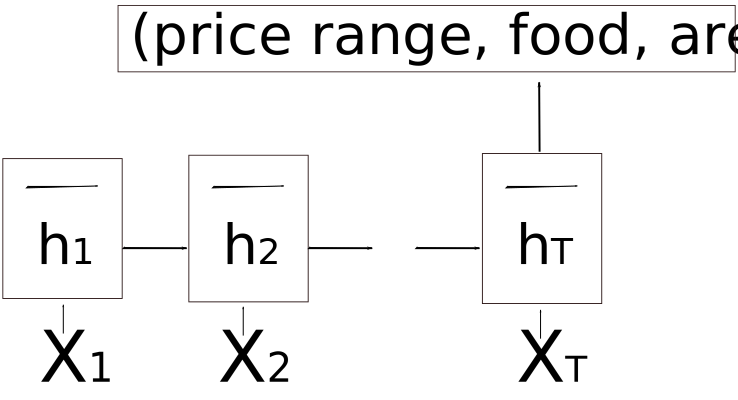
\includegraphics[width=0.5\textwidth]{encoder_joint}
\caption{The joint label predictions using RNN.}
\label{fig:encjoint}
\end{figure}

\subsection{Predicting labels independently}
Independent slots prediction using one classifier per each slot is also very easy to implement.
It does not suffer from curse of dimensionality but it introduce unrealistic assumption of uncorrelated slot properties.
In case of Dstc2 and Cambridge restaurant domain it is hard to believe that slots $area$ and $price range$ do not correlate.
\begin{figure}
\includegraphics[width=0.5\textwidth]{encoder}
\caption{The RNN encodes the word history into dialog state $h_T$ and predicts slot values independently.}
\label{fig:encind}
\end{figure}

\subsection{Encoder decoder framework}
The encoder decoder model with attention\cite{Bahdanout} is the most sophisticated model we used for slot predictions.
To our knowledge we are first who used this model for the task of slot predictions.
The model is typically used in machine translation, does its accuracy does not suffer when predicting longer tuples\cite{Bahdnadou} and it captures correlation between decoded slots easily\cite{LM with attention}.

The disadvantage of this model is its complexity.
First the model is not straight forward to implement\footnote{We modified code from TensorFlow `seq2seq` module.} and also the decoding time is quadratic in length of decoded tuples.
However, we used the model to predict always three labels for first, second and third slot.
\begin{figure}
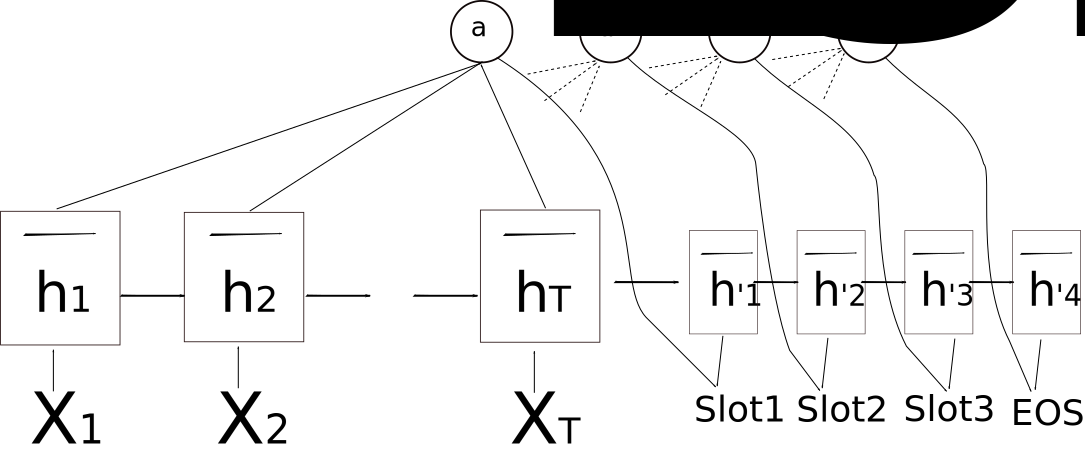
\includegraphics[width=0.5\textwidth]{encdec}
\caption{Encoder decoder with attention predicts goals.}
\label{fig:encdec}
\end{figure}

\section{Experiments}
We report results on the standard split where we used 10\% of data from $train\_dev$ data for early stopping\cite{early stopping} and 90\% for training.
The joint slot accuracy is predicted from \todo{ASR transcription only}.
We report accuracy  on development set which we created and official test set. See~Table~\ref{tab:dstc}.

For all our experiments we use word embeddings of size 40, encoder size of size 50, dropout with keep probability of 0.9.
These parameters where selected after grid search on the parameters.

\subsection{Training}
The training is optimized using cross-entropy loss function and Adam optimizer\cite{todo_adam} with batch size ten.
We train predicting goal slot values at the end of each turn by feeding to the model the turn slot labels $labels_t$ and the whole dialog history until the turn $t$.
Since dialog lengths vary, we employ bucketing of 10 buckets to speed up the computation and we reshuffle the data after each epoch only within a bucket.
Early stopping with patience of four models is run after each epoch on validation set.

\subsection{Labels representation evaluation}
The predicted labels depend often on full history and not only last turn which makes the task very challenging.
Our informal experiments showed that by optimizing the training only on last turn\footnote{The prediction was conditioned on full history but we back-propagated the error only in words for last turn} degrades the performance significantly by more than 40\%. 

Predicting the labels jointly is quite challenging because the distribution of the labels is skewed as demonstrated in~Figure~\ref{fig:labels}.
As some of the labels combinations are very rare they occur only in the development and test set so the joint model is not able to predict them.
We think that such data sparsity of slot triples caused is the root of degraded performance of the joint model.
\begin{figure}
\includegraphics[width=0.5\textwidth]{dstc2_goals_joint_log_scale}
\caption{The histogram of joint labels in the log scale.}
\label{fig:labels}
\end{figure}

The model with independent label prediction obtained much better performance on each slot individually as expected\footnote{TODO report results joint vs independent}, but also it surprisingly outperformed the joint model in the joint prediction.
We think that with larger amount of data the joint model would suffer less from data sparsity and perform better.
This fact is supported by comparing the performance of joint and independent model on the original Dstc2 dataset where training and test set differs much more than on our resplitted version. 
See Table~\ref{tab:dstc} and Table~\ref{tab:resplit} for details.

\begin{table}
\caption{Accuracy on development and {\it Dstc2 test set }}
\begin{center}
\begin{tabular}{r@{\quad}rll}
\hline
\multicolumn{1}{l}{\rule{0pt}{12pt}
                   Model}&\multicolumn{1}{l}{Dev set}&\multicolumn{2}{l}{Test set}\\[2pt]
\hline\rule{0pt}{12pt}
Joint  &     ?&  todo \\
Indep  &   todo& todo \\
EncDec &   todo& todo \\
\hline
\end{tabular}
\end{center}
\label{tab:dstc}
\end{table}

Since the encoder decoder architecture is much more general it needed to learn firstly to predict only three slot labels in the correct order.
It turned out that the architecture learned to predict tuples of four with three slot values and end of string (EOS) symbol quickly even before seeing first half of training data in the first epoch.
At the end of first epoch it made no mistake on predicting slot values in the incorrect order.

The encoder decoder strongly outperformed previous models and the time needed for learning the output structure was surprisingly short
because the best model weights were typically found between fifth and eight epoch for all model configurations including encoder-decoder settings.

\subsection{Data preparation experiments}
As mentioned the data for Dstc2 test set were obtained from another system than the data for validation and training set.\cite{verify and cite dstc2}.
We wanted to investigate how this influence the complexity of the dataset so we merge all Dstc2 data together and created splits of 80\%, 10\% and 10\% for training, development and test set.
The results in Table~\ref{ref:resplit} show that tasked complexity significantly dropped.

\begin{table}
\caption{Accuracy on dev and test set of resplitted Dstc2 data}
\begin{center}
\begin{tabular}{r@{\quad}rll}
\hline
\multicolumn{1}{l}{\rule{0pt}{12pt}
                   Model}&\multicolumn{1}{l}{Dev set}&\multicolumn{2}{l}{Test set}\\[2pt]
\hline\rule{0pt}{12pt}
Joint  &     ?&  todo \\
Indep  &   todo& todo \\
EncDec &   todo& todo \\
\hline
\end{tabular}
\end{center}
\label{tab:repslit}
\end{table}

\section{Related work}
Our system is related to RNN tracker of \cite{Zilka} which reported near state-of-the art result on Dstc2 dataset and was the first incremental system which was able to update the dialog state word-by-word with such accuracy.
In contrast to work of \cite{Zilka} we use no abstraction of slot values but we add the additional features as described in Section~\ref{todo_model_input_featurs}.
The first system which used Neural Network for dialog state tracking \cite{henderson} used feed forward network and manually engineered more than ten features across different levels of abstraction of the user input including spoken language understanding component (SLU).
In our work we focus on simplifying the architecture and so we use only features which are explicitly given by the dialog history word representation and the database.

The system of \cite{Word-based dialog state tracking with recurrent neural networks-Henderson} gives state-of-the-art results and like our system it predicts the dialog state from words using a recurrent neural networks.
On the other hand their system heavily relies on abstracting user input.
Another dialog state tracker with LSTM was used in reinforcement setting but they also used information from SLU pipeline.\cite{Dialog History Construction with Long-Short Term Memory for Robust Generative Dialog State Tracking}

It is worth noting that there are first attempts to train end-to-end dialog system even without explicitly modelling dialog state\cite{Weston} which simplifies the overall architecture of a dialog system.
However, the reported end-to-end model was evaluated only on artificial dataset and cannot be compared to Dstc2 dataset directly.

\section{Conclusion and Future work}
We eval


\subsection*{Future work}
Use standard evaluation metrics on Dstc2 including L2 norm and predict method and requested slots.
Collect and annotate data so we can evaluate the models on another task oriented dataset.




\paragraph{Acknowledgement}
We would like to thank nvidia, gauk, filipgrant.




%
% ---- Bibliography ----
%
\begin{thebibliography}{5}
%
\bibitem {clar:eke}
Clarke, F., Ekeland, I.:
Nonlinear oscillations and
boundary-value problems for Hamiltonian systems.
Arch. Rat. Mech. Anal. {\bf 78} (1982) 315--333

\bibitem {clar:eke:2}
Clarke, F., Ekeland, I.:
Solutions p\'{e}riodiques, du
p\'{e}riode donn\'{e}e, des \'{e}quations hamiltoniennes.
Note CRAS Paris {\bf 287} (1978) 1013--1015

\bibitem {mich:tar}
Michalek, R., Tarantello, G.:
Subharmonic solutions with prescribed minimal
period for nonautonomous Hamiltonian systems.
J. Diff. Eq. {\bf 72} (1988) 28--55

\bibitem {tar}
Tarantello, G.:
Subharmonic solutions for Hamiltonian
systems via a $\bbbz_{p}$ pseudoindex theory.
Annali di Matematica Pura (to appear)

\bibitem {rab}
Rabinowitz, P.:
On subharmonic solutions of a Hamiltonian system.
Comm. Pure Appl. Math. {\bf 33} (1980) 609--633

% JasonDWilliams,“Web-stylerankingandslucombina- tion for dialog state tracking,” in 15th Annual Meeting of the Special Interest Group on Discourse and Dialogue, 2014, p. 282.

\end{thebibliography}
\end{document}
